% Contributors: Tanmay Chopra and Leo Goldman
% May 2020

\section{Fast Approximate Nearest Neighbours} %LEO
\subsection{Background} %Tanmay

\subsubsection{Nearest Neighbours}
The nearest neighbour search problem is defined as follows: \newline
Given a finite set S of points $x_1, x_2...x_n $, and a query point $q $, and a distance metric $d(a,b)$, find the point in set S that is the closest to the queried point.  That is, to find: 
\begin{equation}
    arg min_{x_i \in S}d(x_i,q)
\end{equation}

More commonly, these points are embedded in some sort of geometric space, usually Euclidean, such that $S \in R^d$.\newline
For our purposes, this is usually generalized into the K-nearest neighbours problem - which is simply the extension of the above idea wherein we find the K closest points to the query point, which can be thought of as iteratively performing the above process while removing the $x_i$ returned at each iteration from the set before repeating the process. \newline
This idea is further extended into a classifier for machine learning by adopting a majority vote approach - wherein the label with the greatest multiplicity amongst the K-Nearest Neighbours of a queried point is returned as the result of the classifier for that queried point.  

\subsubsection{Issues with Nearest Neighbour}
While the nearest neighbours classifier is both incredibly effective and intuitive, there are a few issues that arise when implementing this algorithm for large-scale applications.\newline

The first issue arises with an increase in the size of the data set. In the case of the vanilla, brute force method, we iterate through each point in set S and calculate the distance from the queried point to that point. Hence, the computation complexity is linear in the number of samples. As the size of the data set increases, the time taken to compute the nearest neighbours increases. Note that in the brute force method, all these calculations must be carried out for each individual query point. \newline

\begin{figure}[h!]
    \centering
    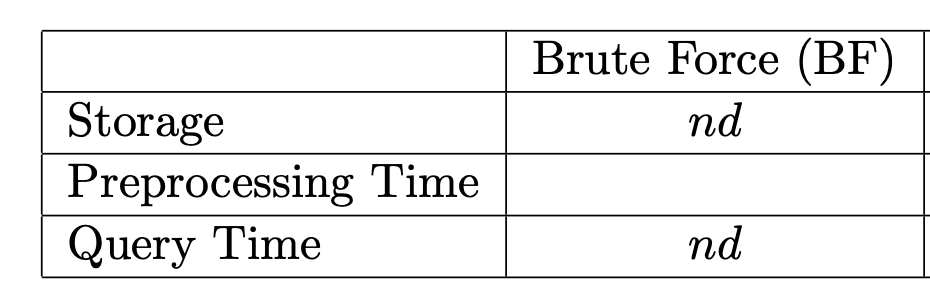
\includegraphics[width=10cm]{chapter_11/files/vanilla.png}
    \caption{Computational Complexity of Vanilla KNN}    
\end{figure}

Another major issue is storage. As we must calculate the distance between the queried points and each given points, we're required to store our whole data set in memory. As data sets scale and we enter the age of big-data, it becomes increasingly challenging to store  entire data set in easily accessible memory locations.\newline

The 'curse of dimensionality' further exacerbates this issue. The data space grows exponentially with the number of dimensions and hence further increases storage requirements. But more importantly, KNN requires points to be close in all dimensions. As dimensions are added, it gets increasingly less likely for points to be definitely close or further away from queried points in all dimensions. \newline

More fundamentally, for non-Euclidian, non-metric spaces, underlying distance measures can take time superlinear to the length of the data. This, coupled with the fact that most indexing methods are not applicable in such spaces, makes efficient nearest neighbour retrieval incredibly complex. 

All these reasons, and many more, have necessitated the search for more computationally feasible solutions to perform nearest neighbour problem, many of which rely on approximation of nearest neighbours over exact ones. 

\subsubsection{Fast ANN introduction}
Since finding nearest neighbors becomes increasingly difficult as the data set grows in size, faster, approximate methods are often looked to as an alternative for finding the actual nearest $k$ neighbors. When querying $q$ for its nearest neighbor, if the output may be off by some threshold, the query time can be dramatically reduced, and in some cases the entire dataset need not be stored, potentially yielding great benefits in space. In some cases, the absolute distance between the approximate nearest neighbor and $q$ can be bounded in terms of $d(x_i,q)$, where $x_i$ is the true nearest neighbor, and in other cases the algorithm finds the nearest neighbor with some probability that is also potentially bounded.

It is important to keep this tradeoff between speed (and possibly space) and accuracy. Although it need not be unique, the nearest neighbor to $q$ always exists and can be found via a linear search among each point's distance to $q$. As mentioned, however, this becomes inefficient and some accuracy is often foregone in exchange for a reduction in query time. Notable improvements occur when one can increase speed or accuracy without sacrificing the other.

The remainder of this section defines certain terminology that is useful in different methods for finding actual or approximate nearest neighbors. Although not all terms are expanded on or used here, Section 2.2 presents structures and algorithms in the literature. In Section 3, we offer examples of fast, approximate nearest neighbor searches found in the literature. 

\subsubsection{Terminology}

\textbf{query}: In any nearest neighbor problem, a query consists of a point, $q$, which is often new to the dataset. Given input $q$, the query outputs the (approximate) nearest neighbor to $q$ in the dataset.

\hfill \break
\noindent
\textbf{c-approximate nearest neighbor problem}: When some amount of error between the actual nearest neighbor and the query output is acceptable, a \emph{c-approximate nearest neighbor} may be acceptable. Rather than $arg min_{x_i \in S}d(x_i,q)$, the c-approximate nearest neighbor is a point, $y_i$, such that $d(y_i,q)\leq c*d(x_i,q)$.

\hfill \break
\noindent
\textbf{$k$-d tree}: A partition of Euclidean space that allows for considering a subset of the entire space when finding nearest neighbors by mainly considering points in the same hyper-rectangular cell.

\hfill \break
\noindent
\textbf{intrinsic dimension}: The smallest number of needed dimensions to create a good representation of the data (need not be exact)

\hfill \break
\noindent
\textbf{random projection trees}: Similar to $k$-d trees, random projection trees (RP trees) partition a Euclidean space. They do so, however, by dividing the space in random directions and by adding noise to the true median in a given direction. [4]

\hfill \break
\noindent
\textbf{spill trees}: Like RP trees, spill trees divide a Euclidean space with randomly chosen directions, but allow for overlap in the sense of a traditional $k$-d tree's cells. The spill tree keeps track of the $.5-\alpha$, .5, and $.5+\alpha$ fractiles of the data along a given directional split, allowing for the possible storage of a point in more than one cell.


\subsection{BoostMap - Machine Learnt Euclidean Embedding for ANNS}

\subsubsection{Embeddings for Fast Approximate Nearest Neighbours} %copied directly, need to edit and structure
The fundamental assumption when creating Euclidean embeddings for data sets is that distance measure is computationally expensive and evaluating distances in Euclidean space is much faster. \newline
In domains where this assumption is applicable, significant computational savings can be obtained by constructing a distance-approximating embedding, which maps objects into another space. \newline
Embeddings are often also used just as a part of the pipeline, as opposed to the complete solution. In these cases, a d-dimensional Euclidean embedding F can be used in a filter-and-refine framework, wherein we preprocess database embeddings offline and then compute the embedding of the queried object. We then filter- finding the p most similar vectors (in the d-dimensional space, wherein distances are measured in $R^d$) and then refine-sorting those candidates by measuring the exact distance between the queried object and eaach candidate. using the original distance measure DX. Hence, the embedding is used to quickly narrow our field of search based on our initial assumption that computing distances in the embedding is faster than in the original space. \newline
Here, p and d can be chosen to optimize for our desired balance between speed and accuracy. As p increases, we are more likely to get the true k nearest neighbors in the top p candidates found at the filter step, but also evaluate more distances at the refine step. Similarly, as d increases, computing the embedding of the queried object becomes more expensive, and measuring distances between vectors in the embedded space also becomes more expensive but we may get more accurate results in the filter step as distortion in the embedded space can be reduced. 

\subsubsection{Solution Overview}
BoostMap is machine learning method for constructing Euclidean embeddings that can be applied to both metric or non-metric spaces. Using AdaBoost, many simple, one dimensional embeddings are combined into a multidimensional embedding that preserves a significant amount of the proximity structure in the original space. BoostMap is most effective in reducing nearest neighbour retrieval time in cases where computing the underlying distance measure is computationally expensive and can take time superlinear to the length of the data. The two main advantages of BoostMap are that it makes no assumptions about the original distance measure and that the construction of the embedding explicitly optimizes a quantitative measure of how well the embedding preserves similarity rankings.

\subsubsection{Measure of Embedding Quality}
In the paper, the authors devise a novel measure of embedding quality focused on nearest neighbour embeddings which aims to preserve the similarity structure of the original space. Let X be a set of objects that comprises the database, q be the queried point and $D_X(x_1,x_2)$ be the distance measure. The proximity order $P_X(q,x_1,x_2)$ is a function defined as follows:

\begin{equation}
 P_X(q,x_1,x_2) = \begin{cases} 1 &\mbox{if } D_X(q,x_1)< D_X(q,x_2)\\
0 &\mbox{if } D_X(q,x_1)= D_X(q,x_2)\\
-1 &\mbox{if } D_X(q,x_1)>D_X(q,x_2)\\\end{cases} 
\end{equation}

Essentially, the function tells us whether q is closer to $x_1$ or $x_2$. Let F be the function that embeds X into $R^d$, hence the associated proximity classifier that determines whether $F(x_1)$ is closer to $F(q)$ or $F(x_2)$ for any triple $(q,x_1,x_2)$ can be defined as follow:

\begin{equation}
    \Tilde{F}(q,x_1,x_2) = D_{R^d}(q,x_1) - D_{R^d}(q,x_2) 
\end{equation}

where $D_{R^d}$ is the distance measure in the embedding. Now we know that sign(x) is 1 for x>0, 0 for x=0 and -1 for x<0, hence we can see that $sign(\Tilde{F}(q,x_1,x_2))$ is an approximation of $P_X$ as defined above. Hence the classification error for a particular classifier on a specific triple can be defined as:

\begin{equation}
    G(\Tilde{F},q,x_1,x_2) = \frac{|P_X(q,x_1,x_2) - sign(\Tilde{F}(q,x_1,x_2))|}{2}
\end{equation}

And the overall error of the classifier is the expected value of G over the set of triples of X.

\begin{equation}
    G(\Tilde{F}) = \frac{\sum_{(q,x_1,x_2) \in X}G(\Tilde{F},q,x_1,x_2)}{|X|^3}
\end{equation}

Constructing an embedding that minimized $G(\Tilde{F})$ intuitively then is an attempt to maintain the similarity structure of X as best as possible as it ensures that $x_1$ is the k-th
nearest neighbor of $x_2$ in X if and only if $F(x_1)$ is the k-th nearest neighbor of $F(x_2)$ in the set F(X) and hence the emphasis is directly on preserving the information that is needed for the nearest neighbour embedding.

\subsubsection{Problem Formulation}
The problem is formulated as an adaptation of AdaBoost as follows:

\begin{itemize}
  \item The training set $T = {(q_1,a_1,b_1),...(q_t,a_t,b_t)}$ consists of a set of t triples of objects in the set X. All triples are created such that q is closer to one of the points - that is, q is not equidistant from the two points. 
  \item $Y={y_1,...y_t}$ is a set of class labels corresponding to each triple, where $y \in {1,-1}$. 
  \item A set $C \subset X$, which are a set of candidate objects used to define 1D embeddings (essentially anchor points from which distances are defined)
  \item A matrix of distances from each c $\in$ C to each $q_i, a_i$ and $b_i$ included in one of the training triples in T
\end{itemize}

Intuitively, the idea is as follows. We have a set of 1-dimensional embeddings which are simply distances from the candidate objects. Each such embedding (relative to each of the candidate points) will have a classifier $\Tilde{F}_j$ associated with it. d (equal to the embedding dimensionality) of these classifiers are crafted into a weighted combination $H = \sum_{j=1}^d \alpha_j \Tilde{F}_j$. The d classifiers (and 1-D embeddings) are chosen from our original set of candidates and weighted to minimize the classification error of H. 
Once we have calculated the optimal classifier H, its component $\Tilde{F}_j$s are used to define a d-dimensional embedding F comprised of all the chosen one-dimensional embeddings and the corresponding weights are used to define a weighted $L_1$ distance. This gives us both the embedding as well as the distance metric for the embedding.

Put simply, we are essentially choosing the optimal d anchor points from the set, measuring distances from them and combining them in a weighting such that we minimize the error to the similarity structure. For any new queried point, we can then measure the distance from these points to get our new embedding and calculate the associated distance metric by weighing the differences in those coordinates between any given points. This is significantly faster than attempting to calculate the distances between all points and each queried object.

\subsubsection{Training Algorithm}
Training occurs in a set of rounds. At each round, the algorithm first attempts to modify a weight of a chosen classifier to reduce the classification error. If such an $a_j$ is found, it is modified. If not, it looks at the set of classifiers not chosen yet, and adds the one that reduces the error the most - that is, it adds the optimal $\Tilde{F}_j$ to H and assigns it the weight that maximises the reduction in error.
By attempting to amend weights BEFORE adding a classifier, the algorithm ensures that the minimum number of classifiers are used and consequently, that the embedding is of lower dimensions for any given accuracy level since each new classifier corresponds to an added dimension and hence minimizes data storage and retrieval time.

To measurthe benefit of choosing a classifier with a specific weight $\alpha$ at the j-th round, we use the following equation:

\begin{equation}
    Z_j((\Tilde{F},\alpha) = \sum_{i=1}^t(w_{i,j}exp(-\alpha y_i \Tilde{F}(q,x_1,x_2))
\end{equation}

Since the benefit increases as the value of this function decreases, at each round we effectively use the following equation:
\begin{equation}
    Z_{min}(B,j) = argmin_{(\Tilde{F},\alpha) \in B X R} Z_j((\Tilde{F},\alpha)
\end{equation}

\subsubsection{Complexity Analysis}
For c candidate objects and n database objects, we compute
cn distances in the original distance metric to learn the embedding and compute the embeddings of all database objects. 
The computational time per training round is O((c + m)t), where t is the number of training triples. In our experiments we always set m = c, that is we have an equal number of pivot pairs and candidate objects.
Computing the d-dimensional embedding of a query object takes O(d) time and requires O(d) evaluations of $D_X$, the original distance metric. 
This can easily be seen to be lower than the computational complexity of the naive nearest neighbours. 

\subsection{Locality-Sensitive Hashing}

\subsubsection{Overview}
This is an algorithmic technique wherein similar items are hashed into the same buckets with high probability and the number of buckets are significantly smaller than the number of objects in the data base. Interestingly enough, unlike usual hashing where we aim to minimize collision, the goal in this case is to maximize them such that we can reduce the dimensionality of high-dimensional data while preserving inter-object distances.


\subsubsection{An LSH Family}
For a given metric space (X,d), scale r>0 and approximation c>1 and a set U, a distribution H over maps $h:X \rightarrow U$ is called $(r,cr,p_1,p_2)$-sensitive if the following holds for any $x \in X$:
\begin{itemize}
  \item if $D(x, y) \leq r$, then $Pr_h[h(x) = h(y)] \geq p_1$
  \item if $D(x, y) \geq cr$, then $Pr_h[h(x) = h(y)] \leq p_2$
\end{itemize}

The  intuition is that an LSH family can be used as a pre-filter for a given data set. Essentially the idea is that for any two points, if the distance between the two points is less than a given threshold (r), the probability that they will hash into the same bucket is greater than or equal to some $p_1$ and if the distance is greater than some scaled value of the threshhold (cr) the probability that they will hash into the same bucket is less than or equal to some $p_2$.
In particular, for a random partition h from the family H, the query point $q$ will likely collide with its near neighbor (with probability at least $p_1$), but with few points at a distance greater than or equal to $cr$, in expectation at most p2 · n of them.

The distribution H is called an LSH family and its quality is measured by $\rho(H) = \frac{\frac{log 1}{p_1}}{\frac{log 1}{p_2}}$

\subsubsection{Algorithm}
For the purposes of this algorithm, we shift our focus from k nearest neighbours to c approximate nearest neighbour, essentially aiming to find a neighbour within the given distance bound. 
Assume we have a family of hash functions as defined above, which can be tailored to one's specific application. 

First, we sample k functions independently from the hash family and produce a combined hash value for each point by concatenating these k hashes. 
\begin{equation}
    g(x) = h_1(x)\cdot h_2(x)...h_k(x)
\end{equation}
Two points are said to collide if $x \neq y $ but $g(x) = g(y)$. Obviously, this can only be this case if $h_i(x) = h_i(y)$ for all $i \in [k]$. Hence,
\begin{itemize}
    \item If $d(x, y) \leq r$ then the probability of collision would be at least $p_1^k$
    \item If $d(x, y) \geq cr$ then the probability of collision would be at most $p_2^k$
\end{itemize}

Hence, k is chosen such that $p_2^k = \frac{1}{n}$ But this makes $p_1$, the probability of colliding with a close point, extremely low. So, we construct $L= n^{\rho}$ different hash tables, each corresponding to its own randomly chosen hash function g. 

In the pre-processing step, all points in X are hashed into each of the L hash tables. On receiving a query point-q, we iterate over the L hash tables. For each table, the data points hashed into the same bucket as q by the corresponding hash function g are retrieved and the distance between each of those points and q is measured i the original metric space, with the process stopping as soon as a point is found to be within distance cr. 

\subsubsection{Guarantees and Complexities}
The following guarantees and complexities can be established.
\begin{itemize}
    \item The probability of finding a point within distance cr, assuming that a point exists within distance r is $1- (1- p_1^k)^L$
    \item $n^{\rho}$ hash tables will be created
    \item Time taken by a query is of the order O($n^{\rho}$)
    \item Space complexity associated with the algorithm is  O($n^{1+\rho}$)
\end{itemize}


\subsection{k-d trees} %Leo

\subsubsection{Solution Overview}
$k$-d trees are a promising tool for finding (approximate) nearest neighbors in a data set that could drastically reduce both the space requirement and query time. A $k$-d tree is a partition of a Euclidean space that is often stored as a binary tree. The tree's root refers to the entire space, and each subsequent child node refers to a subspace of its parent. For a node with two children, the children are separate sets whose union is equivalent to their parent.

\subsubsection{Formulation}
In its simplest form, a $k$-d tree is formed by repeatedly partitioning a space, over a number of directions, at the median of all points in the current cell. In general, the recursive process is as follows:


\begin{algorithm}
\caption{create\_kd\_tree($S, p$)}
\begin{algorithmic} 
\REQUIRE Given a set $S$ and max number of points per cell, $p$
\IF {$|S|\leq p$} \STATE \RETURN $S$ (Leaf node) \ENDIF
\STATE Choose a coordinate direction, $i$
\STATE Define $m:=$median($\{x_i:x\in S\}$)
\STATE Left\_Tree = create\_kd\_tree( $\{x\in S: x_i\leq m\}, p$ )
\STATE Right\_Tree = create\_kd\_tree( $\{x\in S: x_i\geq m\}, p$ )
\STATE \RETURN [ $m$, Left\_Tree, Right\_Tree ]
\end{algorithmic}
\end{algorithm}


Below, is an example of a $k$-d tree in graph and tree form, where the space is divided along the $x$-axis, then $y$-axis, then $x$-axis again, and so on. Note that insertions into the tree are given by the median point, $m$, each time a new tree is created.

\begin{figure}[H]
    \centering
    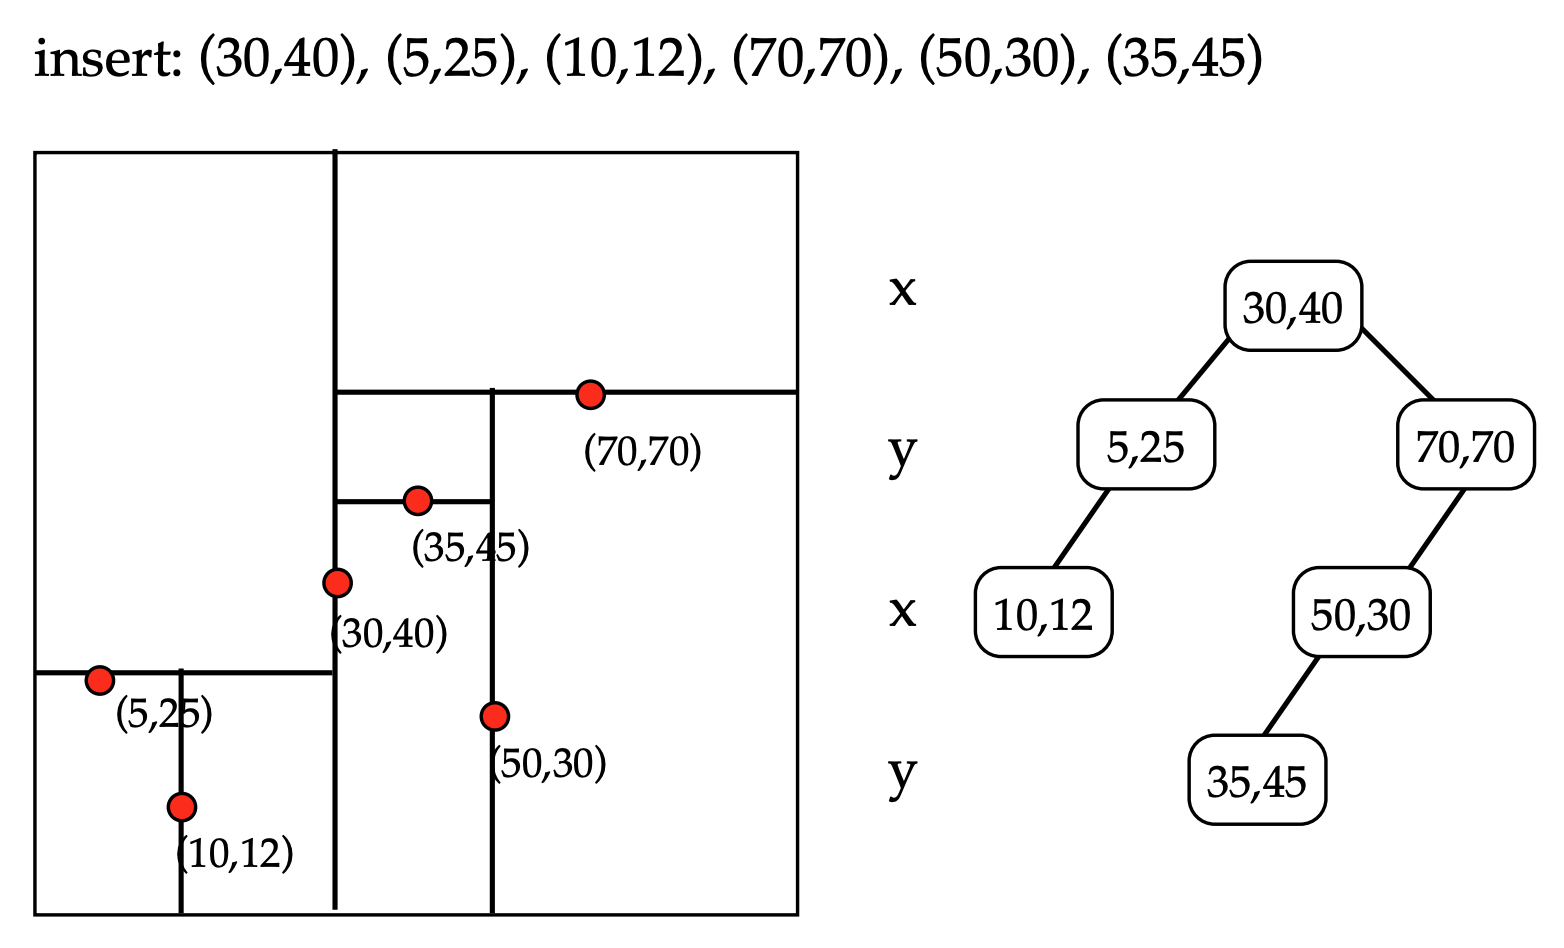
\includegraphics[width=12cm]{chapter_11/files/kd_tree.png}
    \caption{An example $k$-d tree in equivalent forms [3]}
\end{figure}

\subsubsection{Advantages and Disadvantages}
Once a $k$-d tree has been created, it is possible that the dataset need not be stored to find the nearest neighbor in some cases. For example, in classification tasks, each cell can be labeled with the majority label among its points. Then, the labeled partition is just as useful as finding the nearest neighbor(s) for a new point based only on its cell. While limited to the dataset that the tree was created on and other disadvantages of $k$-d trees discussed shortly, this could trivialize the data storage problem. 

Even if, as is typical, the entire dataset is stored, by only considering points in the cell of a queried point, the number of computations can be reduced to a factor of the maximum number of points in each cell. For a fixed $p$, this can be done in $O(log(n))$ time, the order of the tree's depth. More specifically, a query is $O(p+log(n/p))$ or $O(2^d*log(n))$, where $d$ is the dimension of the data, but may be reduced significantly when the dataset has a low intrinsic dimension and only these dimensions are used. This approach, while potentially quick, can suffer from poor accuracy. For example, consdider finding the nearest neighbor to the point (31,71) in the figure above. The nearest neighbor is (35,45), but the nearest point in the same cell as (31,71) is (70,70). For this reason, naïve usage of $k$-d trees can lead to poor performance, and modifications are often necessary. 

\subsection{Improving $k$-d trees and Bounding Failure Probability} 
\subsubsection{Improving on $k$-d trees}
Even though limiting one's search for a nearest neighbor to a $k$-d tree cell can drastically improve query speeds, the insignificant chance of failing to return the actual nearest neighbor creates a need for improved structures and understanding the probability of failure. In the literature, this is often done through two techniques: introducing randomness and allowing for overlap in the traditional $k$-d tree cells.

To introduce randomness to a $k$-d tree, one essentially splits based on random directions, rather than coordinate directions traditionally thought of in Euclidean spaces. In two dimensions, this process creates a structure that looks more like a web as opposed to exclusive rectangles that would make up a traditional $k$-d tree. Furthermore, randomness can be introduced in the splitting decision. While $k$-d trees split along the median in whichever direction is being considered, one could split at some fractile other than .5. This creates a structure akin to a random projection tree, mentioned in Section 2.2, and is more robust to high dimensional data than traditional $k$-d trees. The space requirement for such a tree is linear in the size of teh dataset.

To allow overlap in a $k$-d tree, one creates cells that cover the underlying space but need not be exclusive. In other words, a point can be found in more than one cell or node. To construct such a tree, the space is split in random directions, as above, but now along the median, or .5 fractile, as well as the .5 - $\alpha$ and .5 + $\alpha$ fractiles. By allowing for some amount of overlap, the chances of querying a point that is close to a point in a nearby cell but relatively far from the closest point in its own cell are reduced, for a fixed use case. To keep track of more nodes per point, the space requirement of this structure is 
$O\left(n^{\frac{1}{1-log(1+2\alpha)}}\right)$, which is superlinear in the size of the dataset. Queries are done with a median split moving down the tree, and query times are on the same order as those of traditional $k$-d trees or RP trees. This structure is referred to as a \emph{spill tree}.

In [5], the authors propose a compromise between RP trees and spill trees, called \emph{virtual spill trees}. Like RP trees, virtual spill trees do not allow for overlap in storage, capping the space requirement to $O(n)$. The virtual spill tree, however, essentially allows for overlap in its queries. Each query considers multiple nodes that could contain the nearest neighbor, and finally returns the closest point to $q$ among all points in the union of those cells. The query time, therefore, is increased as compared to RP trees, but the failure probability is reduced. For each of these three structures, the probability of failure for the actual nearest neighbor can be bounded, allowing the user to better understand the tradeoff between speed and accuracy in a nearest neighbor search.

\subsubsection{Bounding Failure Probability}
Unsurprisingly, the probability of failure when using these structures to find the nearest point to $q$ is related to the inherent difficulty of the task. For example, if all points are almost the same distance from $q$, it may be difficult for any structure or algorithm to find the nearest neighbor. At the very least, it is likely that a linear scan cannot be greatly improved on. On the other hand, if one point is close to $q$ and every other point is far from $q$, algorithms with reduced query times should handily outperform a naïve linear scan. It is possible to quantify the difficulty of a given nearest neighbor problem, however, and then use this metric to bound the failure probability for RP, spill, and virtual spill trees [5]. Let $q$ be the query point for which we would like the nearest neighbor and $S=\{x_1,...,x_n\}$ be the dataset from which we would like to find such a neighbor. Furthermore, let $S$ be ordered by distance to $q$ so that $x_1$ is the closest point to $q$ and $x_n$ the furthest.

$$D(q,S)=\frac{1}{|S|}\sum_{i=2}^{|S|}*\frac{\norm{q-x_1}}{\norm{q-x_i}}$$

Let $D\in[0,1]$ be defined as above. Then $D$ is a measure of the problem's difficulty by capturing the average ratio between the actual nearest neighbor to $q$ and each other possible point. It is then possible to use $D$ to bound the probability that $q$ and its actual nearest neighbor, $x_1$ would be placed in separate cells after any division of the current space under consideration when forming a tree. 

After considering the probability that a point, $x_i$ for $i>1$, lands between $q$ and $x_1$ when all points are projected onto a line given by a random direction, the probability that this happens for at least $\alpha$ fraction of the total number of these points is bounded above by:

$$\frac{1}{2\alpha}D(q,S)$$

Since $\alpha$ fraction of these points must be projected in between $q$ and $x_1$ for the two to get separated in such a division of the space, this quantity can be used to bound the probability that $q$ and $x_1$ ever get separated.

For spill trees, recall that $\beta=(1/2)+\alpha$ fraction of points are separated (no overlap) from $1-\beta$ points at each step. Applying the probability that $x_1$ is separated from the eventual cell where $q$ falls, therefore, can be found by summing the probability that this occurs at any step. In other words, let $S'$ contain the $\beta*n$ closest points to $q$, then the probability that $x_1$ is separated from the cell which eventually has $q$ at any given separation is given by $$\frac{1}{2\alpha}*D(q,S')$$
and the probability that this occurs at any given step is given by
$$\frac{1}{2\alpha}*\sum_{i=0}^{L}D(q,S')$$

\noindent
Here, $L$ represents the depth of the spill tree and is equal to $\log_{\frac{1}{\beta}}(n/p)$. For virtual spill trees, the same result holds, but with $\beta =1/2$. When searching for the $k$ nearest neighbors, the probability can simply be multiplied by $k$. 

\noindent
For RP trees, the probability of $x_1$ getting separated from $q$ at any given step is proportional to the equivalent probability in the case of a spill tree, but not exactly the same. The authors of [5] show, however that this probability is bounded by

$$D(q,S_m)*ln(\frac{2e}{D(q,S_m)}$$

where $S_{m_i}$ is the subset of $S$ that contains the $m_i$ closest points to $q$. Recall that at each step in generating a RP tree, a randomly chosen fractile may be chosen to split the current subspace, and let $m_i$ represent that fractile. By taking a union bound over the path from the tree's root to the appropriate leaf for $q$, the overall probability of failure can be bounded by

$$\sum_{i=0}^{L}D(q,S_{m_i})\ln\left(\frac{2e}{D(q,S_{m_i}}\right)$$
\noindent
where $L$ is defined as before.
\newline
\indent
While these probability bounds do not provide determined bounds for the factor by which the output of a query $q$ might be off in the event of failure, they provide a bound on the probability of failure for a search method that may be much quicker than a simple linear scan. In the event that an absolute threshold in the event of failure is needed, previously mentioned methods of nearest neighbor searches may prove more useful.


